% this is a simplified version of 
% https://github.com/yihui/knitr/blob/master/inst/examples/knitr-beamer.Rnw
\documentclass{beamer}\usepackage[]{graphicx}\usepackage[]{color}
%% maxwidth is the original width if it is less than linewidth
%% otherwise use linewidth (to make sure the graphics do not exceed the margin)
\makeatletter
\def\maxwidth{ %
  \ifdim\Gin@nat@width>\linewidth
    \linewidth
  \else
    \Gin@nat@width
  \fi
}
\makeatother

\definecolor{fgcolor}{rgb}{0.345, 0.345, 0.345}
\newcommand{\hlnum}[1]{\textcolor[rgb]{0.686,0.059,0.569}{#1}}%
\newcommand{\hlstr}[1]{\textcolor[rgb]{0.192,0.494,0.8}{#1}}%
\newcommand{\hlcom}[1]{\textcolor[rgb]{0.678,0.584,0.686}{\textit{#1}}}%
\newcommand{\hlopt}[1]{\textcolor[rgb]{0,0,0}{#1}}%
\newcommand{\hlstd}[1]{\textcolor[rgb]{0.345,0.345,0.345}{#1}}%
\newcommand{\hlkwa}[1]{\textcolor[rgb]{0.161,0.373,0.58}{\textbf{#1}}}%
\newcommand{\hlkwb}[1]{\textcolor[rgb]{0.69,0.353,0.396}{#1}}%
\newcommand{\hlkwc}[1]{\textcolor[rgb]{0.333,0.667,0.333}{#1}}%
\newcommand{\hlkwd}[1]{\textcolor[rgb]{0.737,0.353,0.396}{\textbf{#1}}}%
\let\hlipl\hlkwb

\usepackage{framed}
\makeatletter
\newenvironment{kframe}{%
 \def\at@end@of@kframe{}%
 \ifinner\ifhmode%
  \def\at@end@of@kframe{\end{minipage}}%
  \begin{minipage}{\columnwidth}%
 \fi\fi%
 \def\FrameCommand##1{\hskip\@totalleftmargin \hskip-\fboxsep
 \colorbox{shadecolor}{##1}\hskip-\fboxsep
     % There is no \\@totalrightmargin, so:
     \hskip-\linewidth \hskip-\@totalleftmargin \hskip\columnwidth}%
 \MakeFramed {\advance\hsize-\width
   \@totalleftmargin\z@ \linewidth\hsize
   \@setminipage}}%
 {\par\unskip\endMakeFramed%
 \at@end@of@kframe}
\makeatother

\definecolor{shadecolor}{rgb}{.97, .97, .97}
\definecolor{messagecolor}{rgb}{0, 0, 0}
\definecolor{warningcolor}{rgb}{1, 0, 1}
\definecolor{errorcolor}{rgb}{1, 0, 0}
\newenvironment{knitrout}{}{} % an empty environment to be redefined in TeX

\usepackage{alltt}
\IfFileExists{upquote.sty}{\usepackage{upquote}}{}
\begin{document}

\title{Introducci\'on a la Gen\'omica \\ UNAL nov 2017}
\author{Alejandro Caceres \\ ISGlobal, Barcelona}


\maketitle

% very important to use option [fragile] for frames containing code output!

\begin{frame}[fragile]
\frametitle{Control de Calidad}
Los datos de microarrays son sometidos un control de calidad
\begin{itemize}

\item {\tt SNPs}: Calidad del genotipado o que biol\'ogimcamente no correspondan a lo esperado 

\item {\tt Sujetos}: Sujetos que son ''outliers´´ de la muestra: ancestr\'ia o parentesco 

\end{itemize}
\end{frame}

\begin{frame}[fragile]
\frametitle{Genotipado}
En illumina los datos crudos son las intensidades de cada alelo

\begin{figure}[htbp]
\begin{center}
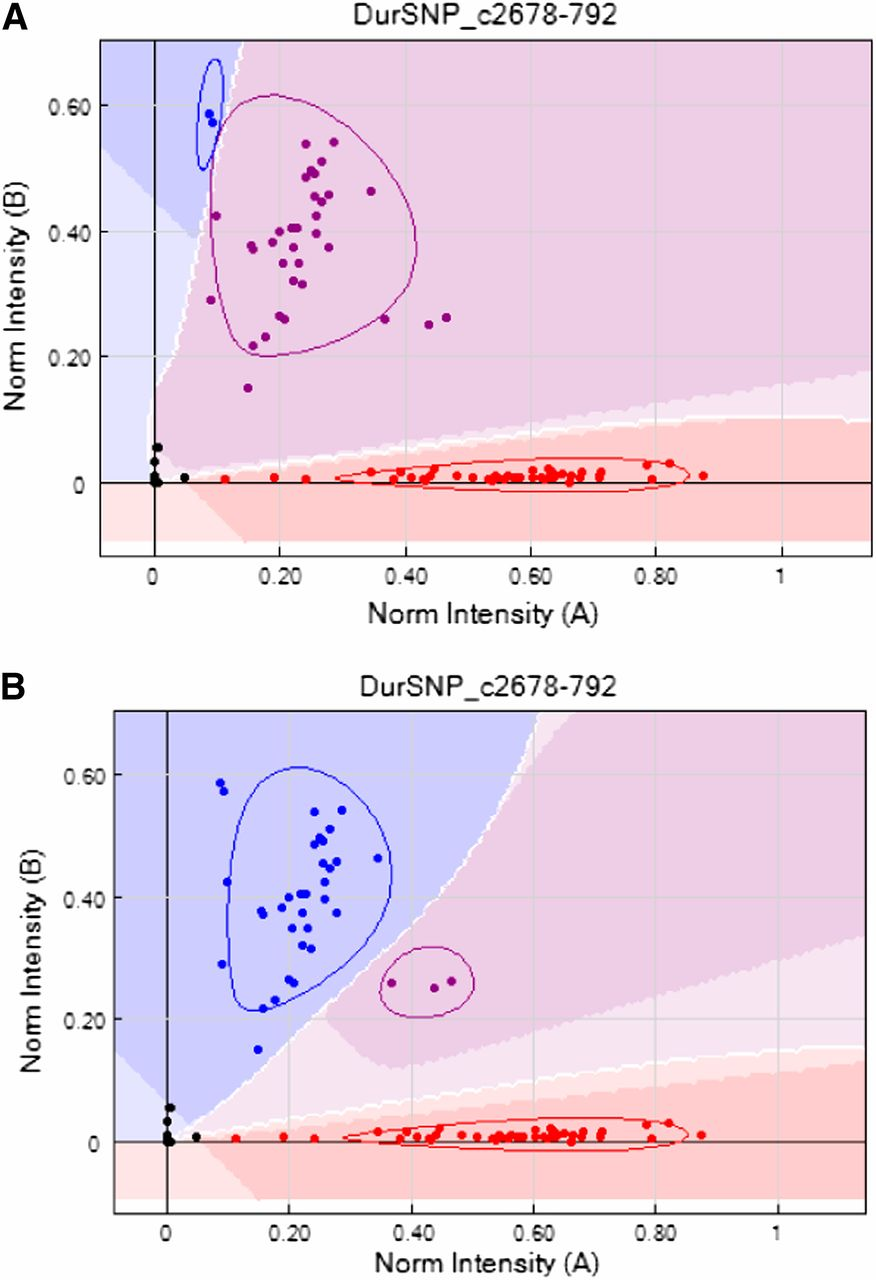
\includegraphics[width=.5\linewidth]{clustermicro.jpg}
\end{center}
\end{figure}

entre menos varianza en angulo entre los grupos mejor es la genotipacion del SNP

\begin{itemize}
\item B-allelefreq: la intensidad relativa del allelo B respecto al A (angulo)
\item log2ratio: la intensidad de la observacion respecto al grupo (magnitud)
\end{itemize}

\end{frame}



\begin{frame}[fragile]
\frametitle{GenomeStudio}

Es el software de Illumina para hacer el genotipado de los SNPs (clustering)
\begin{figure}[htbp]
\begin{center}
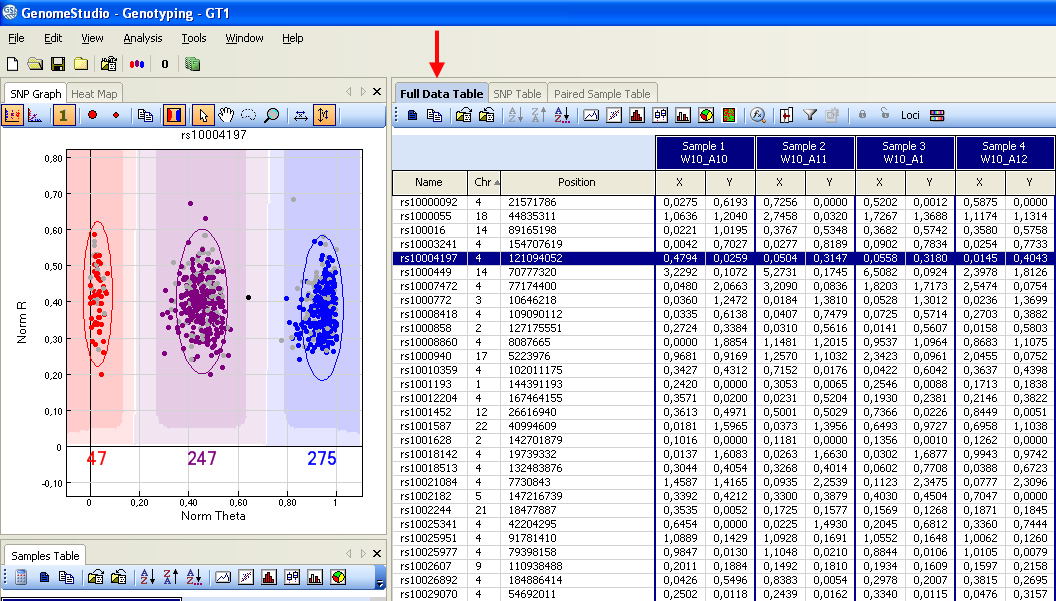
\includegraphics[width=.6\linewidth]{genomestudio.jpg}
\end{center}
\end{figure}

\begin{itemize}
\item el control de calidad en el genotipado est\'a dado por el clustering
\item reporta un calldate y un valor del numero de sujetos con genotipado aceptable por SNP 
\item genera los genotipos en formato PLINK 
\end{itemize}

\end{frame}


\begin{frame}[fragile]
\frametitle{Control de Calidad por Sujetos}

\begin{itemize}
\item que el sexo es el reportado o detecci\'on de aneploidías como XXY, XYY, etc 
\item cosanginidad mas alta de la esperado en el diseño del estudio 
\end{itemize}

\end{frame}


\begin{frame}[fragile]
\frametitle{Identidad por descendencia}

La consanginidad (identity by descent) se puede calcular en PLINK por medio de la opci\'on --genome

\begin{verbatim}
acaceres@IMW00680:~$ plink --bfile [filename prefix] --genome 
\end{verbatim}

y produce un reporte en el fichero {\tt plink.genome}
\end{frame}



\begin{frame}[fragile]
\frametitle{Control de calidad de SNPs}

\begin{itemize}
\item Call-rate (dada por genomeStudio): $>80\%$
\item Minor allele frequency (MAF): $>0.01$ o $>0.05$
\item Hardy Weinberg Equillibrium: menos de 3 o 4 desviaciones standard 
\item Mendelian errors: si hay trios que no tengan errores de trasmisi\'on
\end{itemize}

\end{frame}

\begin{frame}[fragile]
\frametitle{Equilibrio de Hardy Weinberg}

En una poblaci\'on en donde no hay fuerzas que cambien la frecuencia alelica $p$ (de un SNP)
debemos encontar
\begin{itemize}
\item $p^2$ fracci\'on de homicigotos
\item $2*p*(p-1)$ fracci\'on de heretocigotos
\item $(1-p)^2$ fracci\'on de homocigotos variantes
\end{itemize}

que se deducen por la asociaci\'on aleatoria entre los cromosomas paternos y maternos


\end{frame}



\begin{frame}[fragile]
\frametitle{Equilibrio de Hardy Weinberg}

SNPs que no est\'an en WHE pueden presentar

\begin{itemize}
\item Problemas de genotipaci\'on. Por ejemplo una sonda defectuosa en la mitad de la población (Alta disviaci\'on-Probable).
\item Fuerzas evolutivas sobre el SNP (Baja disviaci\'on-Menons probable)).
\end{itemize}

Si la desviación en biol\'ogica como en el segundo caso, SNPs vacinos que estan en LD tambi\'en deben estar desviados. 

\end{frame}

\begin{frame}[fragile]
\frametitle{Errores Mendelianos}
Para un estudio con trios los SNPs de 
\begin{itemize}
\item dos padres homocigotos para el mismo alelo no pueden tener un hijo que no sea homocigoto
\item un padre homocigoto y una madre heterocigota no pueden tener un hijo que no sea homocigoto alternativo
\item un padre homocigoto para un alelo y una madre homocigota para el otro alele no pueden tener un hijo homocigoto para ning\'un alelo 
\end{itemize}

desviaciones en estas reglas son herrores de trasmisi\'on mendelianos e indican error en genotipaci\'on

\end{frame}



\begin{frame}[fragile]
\frametitle{Software}

\begin{itemize}
\item el control de calidad para MAF, HWE y call-rate se puede hacer con la mayor\'ia de paquertes
\item veamos como se have con SNPstats
\end{itemize}

En R cargemos la librer\'ia y los datos
\begin{knitrout}\footnotesize
\definecolor{shadecolor}{rgb}{0.969, 0.969, 0.969}\color{fgcolor}\begin{kframe}
\begin{alltt}
\hlkwd{library}\hlstd{(}\hlstr{"snpStats"}\hlstd{)}
\end{alltt}


{\ttfamily\noindent\itshape\color{messagecolor}{\#\# Loading required package: survival}}

{\ttfamily\noindent\itshape\color{messagecolor}{\#\# Loading required package: Matrix}}\begin{alltt}
\hlkwd{load}\hlstd{(}\hlstr{"datos/snpsSNPstats.RData"}\hlstd{)}
\hlstd{snpsSNPstats}
\end{alltt}
\begin{verbatim}
## A SnpMatrix with  2504 rows and  1863 columns
## Row names:  HG00096 ... NA21144 
## Col names:  rs555347111 ... rs558158882
\end{verbatim}
\end{kframe}
\end{knitrout}
\end{frame}


\begin{frame}[fragile]
\frametitle{SNPStats}
{\tt col.summary} calcula call-rate, MAF, HWE para todos los SNPs en la base de datos
\begin{knitrout}\footnotesize
\definecolor{shadecolor}{rgb}{0.969, 0.969, 0.969}\color{fgcolor}\begin{kframe}
\begin{alltt}
\hlstd{sum} \hlkwb{<-} \hlkwd{col.summary}\hlstd{(snpsSNPstats)}
\hlkwd{dim}\hlstd{(sum)}
\end{alltt}
\begin{verbatim}
## [1] 1863    9
\end{verbatim}
\begin{alltt}
\hlkwd{head}\hlstd{(sum)}
\end{alltt}
\begin{verbatim}
##             Calls Call.rate Certain.calls         RAF         MAF
## rs555347111  2504         1             1 0.073682109 0.073682109
## rs573543994  2504         1             1 0.012180511 0.012180511
## rs542617372  2504         1             1 0.076078275 0.076078275
## rs562398147  2504         1             1 0.011781150 0.011781150
## rs576107214  2504         1             1 0.021365815 0.021365815
## rs188856175  2504         1             1 0.008785942 0.008785942
##                  P.AA        P.AB        P.BB      z.HWE
## rs555347111 0.8554313 0.141773163 0.002795527   1.930779
## rs573543994 0.9796326 0.016373802 0.003993610 -15.991828
## rs542617372 0.8582268 0.131389776 0.010383387  -3.271542
## rs562398147 0.9844249 0.007587859 0.007987220 -33.733301
## rs576107214 0.9740415 0.009185304 0.016773163 -39.048892
## rs188856175 0.9848243 0.012779553 0.002396166 -13.324690
\end{verbatim}
\end{kframe}
\end{knitrout}
\end{frame}

\begin{frame}[fragile]
\frametitle{SNPStats}
obtengamos los SNPs con call-rate >0.8
\begin{knitrout}\footnotesize
\definecolor{shadecolor}{rgb}{0.969, 0.969, 0.969}\color{fgcolor}\begin{kframe}
\begin{alltt}
\hlstd{Callrate} \hlkwb{<-} \hlstd{sum}\hlopt{$}\hlstd{Call.rate}
\hlstd{selectCallRate} \hlkwb{<-} \hlstd{Callrate} \hlopt{>} \hlnum{0.8}
\hlkwd{length}\hlstd{(selectCallRate)}
\end{alltt}
\begin{verbatim}
## [1] 1863
\end{verbatim}
\begin{alltt}
\hlkwd{head}\hlstd{(selectCallRate)}
\end{alltt}
\begin{verbatim}
## [1] TRUE TRUE TRUE TRUE TRUE TRUE
\end{verbatim}
\end{kframe}
\end{knitrout}
\end{frame}


\begin{frame}[fragile]
\frametitle{SNPStats}
obtengamos los SNPs con frequencia mayor a 0.01
\begin{knitrout}\footnotesize
\definecolor{shadecolor}{rgb}{0.969, 0.969, 0.969}\color{fgcolor}\begin{kframe}
\begin{alltt}
\hlstd{MAF} \hlkwb{<-} \hlstd{sum}\hlopt{$}\hlstd{MAF}
\hlstd{selectMAF} \hlkwb{<-} \hlstd{MAF} \hlopt{>} \hlnum{0.01}
\hlkwd{length}\hlstd{(selectMAF)}
\end{alltt}
\begin{verbatim}
## [1] 1863
\end{verbatim}
\begin{alltt}
\hlkwd{head}\hlstd{(selectMAF)}
\end{alltt}
\begin{verbatim}
## [1]  TRUE  TRUE  TRUE  TRUE  TRUE FALSE
\end{verbatim}
\end{kframe}
\end{knitrout}
\end{frame}


\begin{frame}[fragile]
\frametitle{SNPStats}
Cuales SNPs tienen $MAF>0.01$ y $CallRate > 0.80$
\begin{knitrout}\footnotesize
\definecolor{shadecolor}{rgb}{0.969, 0.969, 0.969}\color{fgcolor}\begin{kframe}
\begin{alltt}
\hlstd{selectMAFCAllrete} \hlkwb{<-} \hlstd{selectMAF} \hlopt{&} \hlstd{selectCallRate}
\hlkwd{head}\hlstd{(selectMAFCAllrete)}
\end{alltt}
\begin{verbatim}
## [1]  TRUE  TRUE  TRUE  TRUE  TRUE FALSE
\end{verbatim}
\begin{alltt}
\hlkwd{table}\hlstd{(selectMAFCAllrete)}
\end{alltt}
\begin{verbatim}
## selectMAFCAllrete
## FALSE  TRUE 
##   420  1443
\end{verbatim}
\end{kframe}
\end{knitrout}

\begin{knitrout}\footnotesize
\definecolor{shadecolor}{rgb}{0.969, 0.969, 0.969}\color{fgcolor}\begin{kframe}
\begin{alltt}
\hlstd{snpnames} \hlkwb{<-} \hlkwd{colnames}\hlstd{(snpsSNPstats)}
\hlkwd{length}\hlstd{(snpnames)}
\end{alltt}
\begin{verbatim}
## [1] 1863
\end{verbatim}
\begin{alltt}
\hlkwd{head}\hlstd{(snpnames)}
\end{alltt}
\begin{verbatim}
## [1] "rs555347111" "rs573543994" "rs542617372" "rs562398147" "rs576107214"
## [6] "rs188856175"
\end{verbatim}
\begin{alltt}
\hlstd{selsnpnames} \hlkwb{<-} \hlstd{snpnames[selectMAFCAllrete]}
\hlkwd{length}\hlstd{(selsnpnames)}
\end{alltt}
\begin{verbatim}
## [1] 1443
\end{verbatim}
\begin{alltt}
\hlkwd{head}\hlstd{(selsnpnames)}
\end{alltt}
\begin{verbatim}
## [1] "rs555347111" "rs573543994" "rs542617372" "rs562398147" "rs576107214"
## [6] "rs17763596"
\end{verbatim}
\end{kframe}
\end{knitrout}
\end{frame}


\begin{frame}[fragile]
\frametitle{SNPStats}
teniendo los SNPs se puede seleccionar una submatriz de los genotipos con s\'olo estos SNPs
\begin{knitrout}\footnotesize
\definecolor{shadecolor}{rgb}{0.969, 0.969, 0.969}\color{fgcolor}\begin{kframe}
\begin{alltt}
\hlstd{NewsnpsSNPstats}\hlkwb{<-}\hlstd{snpsSNPstats[,selsnpnames]}
\hlstd{NewsnpsSNPstats}
\end{alltt}
\begin{verbatim}
## A SnpMatrix with  2504 rows and  1443 columns
## Row names:  HG00096 ... NA21144 
## Col names:  rs555347111 ... rs558158882
\end{verbatim}
\end{kframe}
\end{knitrout}
\end{frame}


\begin{frame}[fragile]
\frametitle{Ejercicio}

\begin{itemize}
\item Seleccionar ahora los SNPs que tienen $abs(sum\$z.HWE) < 6$
\item Crear una nueva matriz con los SNPs seleccionados
\end{itemize}

desviaciones en estas reglas son herrores de trasmisi\'on mendelianos e indican error en genotipaci\'on
\end{frame}

\begin{frame}[fragile]
\frametitle{ejercicio}
\begin{knitrout}\footnotesize
\definecolor{shadecolor}{rgb}{0.969, 0.969, 0.969}\color{fgcolor}\begin{kframe}
\begin{alltt}
\hlstd{selhw}\hlkwb{<-}\hlkwd{abs}\hlstd{(sum}\hlopt{$}\hlstd{z.HWE)} \hlopt{<} \hlnum{6}
\hlstd{NewsnpsSNPstats}\hlkwb{<-}\hlstd{snpsSNPstats[, selhw} \hlopt{&} \hlstd{selectMAF} \hlopt{&} \hlstd{selectCallRate]}
\hlkwd{save}\hlstd{(NewsnpsSNPstats,} \hlkwc{file}\hlstd{=}\hlstr{"NewsnpsSNPstats.RData"}\hlstd{)}
\end{alltt}
\end{kframe}
\end{knitrout}
\end{frame}




\end{document}
